
\documentclass[11pt]{article}

\usepackage{lineno}
\linenumbers

\usepackage[a4paper, margin=1in]{geometry}
%\usepackage{cite}
\usepackage[square]{natbib} % <- new

\usepackage{datetime}
\usepackage{xcolor}
\usepackage{amsmath}  % for \rvert and \lvert
\usepackage{graphicx}


%\longdate

\usepackage{titlesec}
\titleformat*{\section}{\large\bfseries}

\usepackage{parskip}
\setlength{\parindent}{0pt}

\begin{document}

\title{\textit{Title: something about local hydronamics determined by reef lagoon... biophysical feedback/control/influence, breaking-wave water level setup...}}
\author{}
%\affiliation{Various universities}

\date{\today}

\maketitle

\begin{abstract}
Abstract here
\end{abstract}

\section{Introduction}

\begin{itemize}
	\item Importance of coral reefs, barrier islands, etc. (including \citep{guannel16})
	\item Coral reef hydrodynamics (e.g. \citep{gourlay96, symonds05})
	\item Coral reef lagoon hydrodynamics
	\item Caribbean lagoon dynamics? (e.g. \citep{ocallaghan07})
	\item Inlets and waves? (e.g. we know wave setup adjusts the tide/water level in shallow inlets \citep{williams16})
\end{itemize}

\section{Methods}



\subsection{Site background and field measurements}
\subsubsection{Background on Laguna Nichupt{\'e} and the local reefs}

\citet{merino90} made measurements in 1982 and 1983 in the lagoon. \citet{pedrozoacuna08} did a modeling study for a Masters project. \citet{romerosierra18} also did a MS project in the lagoon. They made measurements in the ``rainy'' and ``cold front'' seasons of water quality parameters, temperature, salinity, and used bathymetry and winds to look at circulation. This study appears to have treated the inlets as closed (thus the system responded only to wind, freshwater discharge, and evaporation), but gives important recent measurements of nutrient and DO in the NLS. Oxygen and eutrophication in Bojorquez \citep{reyes91}, on tourism in the area \citep{torres05}, more eutrophication in response to tourism \citep{merino92}, zooplankton in Bojorquez \citep{alvarezcadena96}, sediment oxygen demand in Bojorquez \citep{valdeslozano06}. 

\textcolor{magenta}{Figure (here or in results): Showing water level setup by the reef lagoon - can we compare to the other side of Nichupte?}

\subsection{Field study}

A 24-hour field study was performed 

\textcolor{magenta}{Figure needed: Map of the region with locations of the measurements}

\textcolor{magenta}{Figure needed: Conditions during study: Wave climate, wind speed and direction, air temperature? some indication of freshwater flow into the lagoon if possible?}


\subsection{Idealized numerical model}

\begin{itemize}
	\item Model used
	\item Idealization how (non-dimensionalization? How does it match to the actual conditions)
	\item Forcing
		\item Wind
		\item Waves
		\item Coastal current
\end{itemize}

\textcolor{magenta}{Figure needed: Map of the idealized model}


\section{Results}

\begin{itemize}
	\item Northward flow: compare water level at two inlets and currents at two inlets
	\item Salinity data (saltier, well-mixed at South, stratified, fresher at north - figures~\ref{figDensityNizuc})
	\item Harmonic analysis - seiche (from the reef lagoon, I think)
\end{itemize}

\textcolor{magenta}{Figures needed: Water levels (figure~\ref{figWLnizuc}, water velocities, harmonic analysis}



\section{Discussion}

\textit{Do the model results go in Results or Discussion?}

Figure~\ref{figSeiche} shows seiches periods given varying lagoon lengthscales. 




\section{Conclusions}


\section{Acknowledgement}

\textit{[Insert here: funding details, field help from 20-odd students in Introduction to the dynamics of semienclosed bodies of water summer course, etc.]}



\bibliography{nichupte}{}
\bibliographystyle{apalike}

% FIGURES HERE
\begin{figure}[ht!]
\centerline{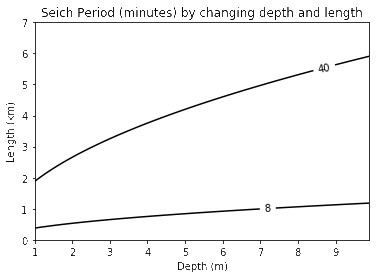
\includegraphics[width=0.5\textwidth]{images/nichupteseiche.png}}

\internallinenumbers\caption{Seiche period \textcolor{magenta}{open or closed lagoon? $\frac{2 L}{\left(gH\right)^{1/2}}$ or $\frac{4 L}{\left(gH\right)^{1/2}}$}}
\label{figSeiche}
\end{figure}


\begin{figure}[ht!]
\centerline{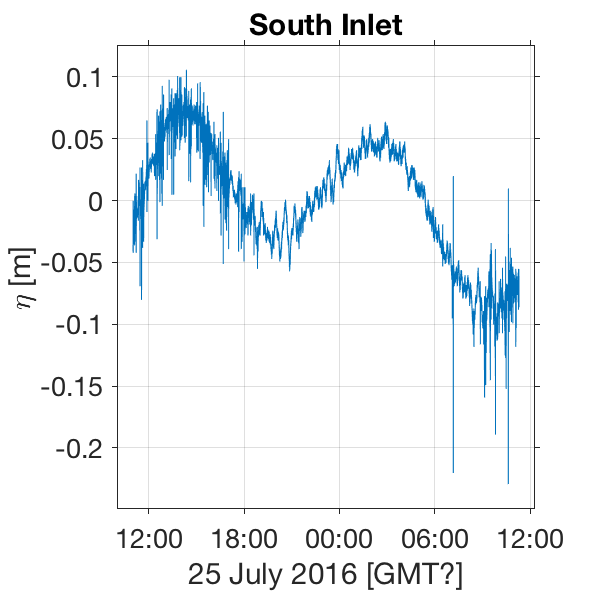
\includegraphics[width=0.5\textwidth]{images/waterlevel_southinlet.png}}
\internallinenumbers\caption{Placeholder, south inlet water level}
\label{figWLnizuc}
\end{figure}

\begin{figure}[ht!]
\centerline{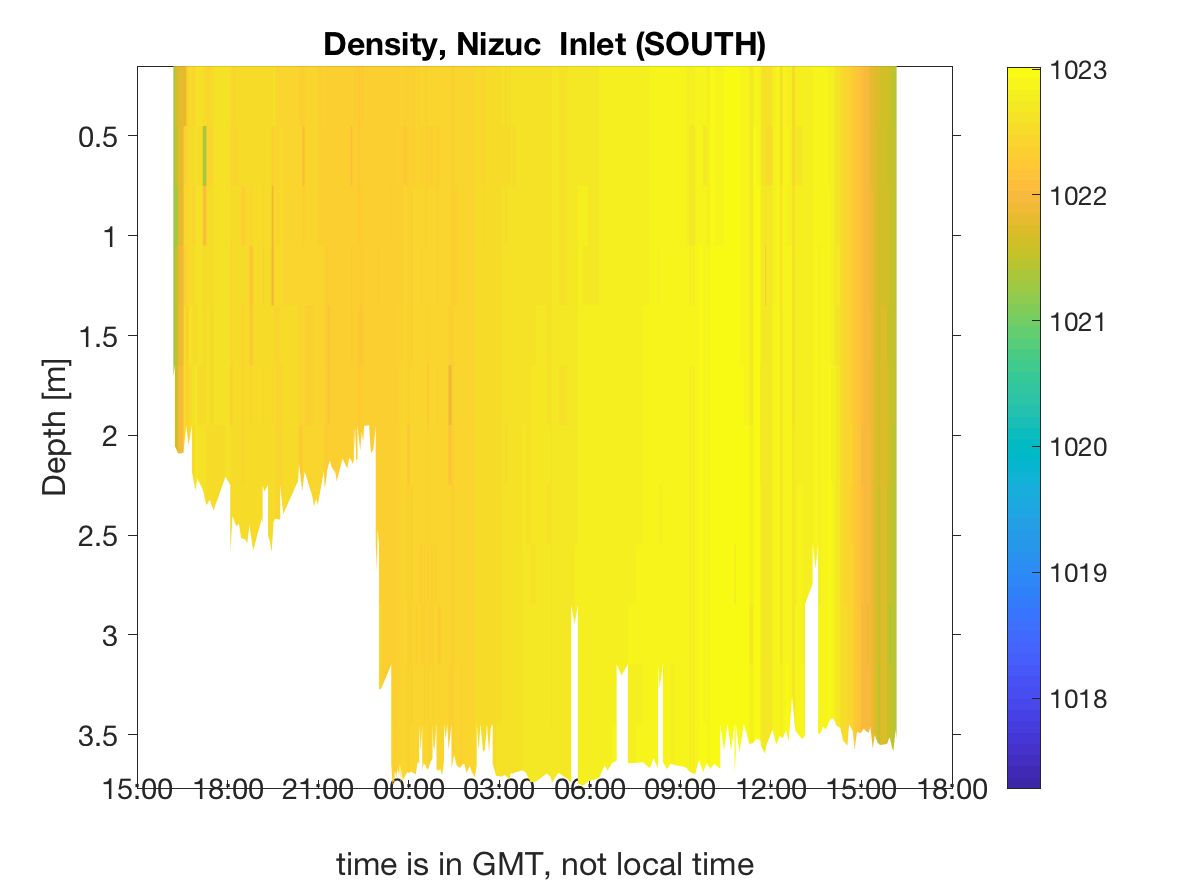
\includegraphics[width=0.5\textwidth]{images/density_nizuc_nichupte_southinlet.png}}
\internallinenumbers\caption{Placeholder, density at the South inlet}
\label{figDensityNizuc}
\end{figure}



\end{document}